\documentclass[10.5pt]{article}
\usepackage{amsmath,amssymb,amsthm}
\usepackage{amsfonts,bm}
\usepackage{listings}
\usepackage{graphicx}
\usepackage[shortlabels]{enumitem}
\usepackage{tikz}
\usepackage{extramarks}
%\usepackage{enumerate}
\usepackage[margin=1in]{geometry}
\usepackage{fancyhdr}
\usepackage{epsfig}
\usepackage{amsmath}
\usepackage{float}
\usepackage{amssymb}
\usepackage{caption}
\usepackage{subfigure}
\usepackage{graphics}
\usepackage{titlesec}
\usepackage{mathrsfs}
\usepackage{amsfonts}
\usepackage{indentfirst}
\usepackage{fontspec}
\usepackage{dashrule}
\usepackage{ctex}
\usepackage{algpseudocode}
%\usepackage{algorithm}

\renewcommand{\baselinestretch}{1.2}

\usepackage{tikz-qtree}
\usetikzlibrary{graphs}
\tikzset{every tree node/.style={minimum width=2em,draw,circle},
	blank/.style={draw=none},
	edge from parent/.style=
	{draw,edge from parent path={(\tikzparentnode) -- (\tikzchildnode)}},
	level distance=1.2cm} 
\setlength{\parindent}{0pt}
\setlength{\headheight}{13.6pt}
\newcommand\question[1]{\vspace{.2in}\hrule\vspace{0.04in}\textbf{Problem\ #1}\vspace{.4em}\hrule\vspace{.10in}}
\newcommand\Solution{\vspace{.3in}\textbf{Solution:}\vspace{.5em}\hrule\vspace{.08in}\par}
\newcommand\Answer{\vspace{.2in}\textbf{Answer:}\vspace{.5em}\hrule\vspace{.08in}\par}
\newcommand\Proof{\vspace{.3in}\textbf{Proof:}\vspace{.5em}\hrule\vspace{.08in}\par}
\newcommand\minsolution{\vspace{.3in}\textbf{Solution:}\vspace{.4em}\par}
\newcommand\minanswer{\vspace{.2in}\textbf{Answer:}\vspace{.4em}\par}
\newcommand\minproof{\vspace{.3in}\textbf{Proof:}\vspace{.4em}\par}
\renewcommand\part[1]{\vspace{.10in}\textbf{(#1)}}
\newcommand\algorithm{\vspace{.10in}\textbf{Algorithm: }}
\newcommand\correctness{\vspace{.10in}\textbf{Correctness: }}
\newcommand\runtime{\vspace{.10in}\textbf{Running time: }}
\pagestyle{fancyplain}

\setCJKfamilyfont{Song}[AutoFakeBold]{宋体-简 细体}
\newcommand*{\Song}{\CJKfamily{Song}}




\newcommand{\horrule}[1]{\rule{\linewidth}{#1}}

\title{
	\normalfont \normalsize
	\begin{figure}[!h]
	\centering
	
\includegraphics[width=4.8in, keepaspectratio]{logo_red.pdf}\\[1cm]
		%\caption{}
	\end{figure}
	%\huge{\textsc{ShanghaiTech University}} \\ [8pt]
	\horrule{0.5pt} \\[0.4cm]
	\Huge SI140 Probability \& Mathematical Statistics\\[0.4cm]
	\LARGE Homework 11\\
	\horrule{2pt} \\[1.5cm]
}
 
\author{\Song{\huge\textbf{陈昱聪}}\\[0.2cm]Chen Yucong\ ><E<>N\\[4.5cm]\textbf{Student ID: 2019533079}\\[0.2cm] 
\textbf{Email:}\ {\ttfamily chenyc@shanghaitech.edu.cn}\\[0.8cm] \LARGE\textsc{School of Information Science and Technology}\\[0.63cm]
\texttt{$\circledcirc$ Group\#2\ (TA:曾理)}}
\date{}


\pagestyle{fancy}
\lhead{SI140 Probability \& Mathematical Statistics}
\chead{\textbf{Homework 11\ }}
\rhead{陈昱聪\,2019533079\ \,Due:\,11:59\,am, $14^{\text{th}}$ Dec.}
\cfoot{\thepage}
\renewcommand{\headrulewidth}{0.4pt}


\fancypagestyle{firstpage}
{
	\renewcommand{\headrulewidth}{0pt}
	\fancyhf{}
	\fancyfoot[C]{\thepage}
}


\newcounter{ProblemCounter}
\newcounter{oldvalue}
\newcommand{\problem}[2][-1]{
	\setcounter{oldvalue}{\value{secnumdepth}}
	\setcounter{secnumdepth}{0}
	\ifnum#1>-1
	\setcounter{ProblemCounter}{0}
	\else
	\stepcounter{ProblemCounter}
	\fi
	\section{Problem \arabic{ProblemCounter}: #2}
	\setcounter{secnumdepth}{\value{oldvalue}}
}
\newcommand{\subproblem}[1]{
	\setcounter{oldvalue}{\value{section}}
	\setcounter{section}{\value{ProblemCounter}}
	\subsection{#1}
	\setcounter{section}{\value{oldvalue}}
}

\setmonofont{Helvetica}
\definecolor{blve}{rgb}{0.3372549 , 0.61176471, 0.83921569}
\definecolor{gr33n}{rgb}{0.29019608, 0.7372549 , 0.64705882}
\makeatletter
\lst@InstallKeywords k{class}{classstyle}\slshape{classstyle}{}ld
\makeatother
\lstset{language=C++,
	basicstyle=\ttfamily,
	keywordstyle=\color{blve}\ttfamily,
	stringstyle=\color{red}\ttfamily,
	commentstyle=\color{green}\ttfamily,
	morecomment=[l][\color{magenta}]{\#},
	classstyle = \bfseries\color{gr33n}, 
	tabsize=4
}


\begin{document}
	
\maketitle
\thispagestyle{firstpage}
\thispagestyle{empty}
\setcounter{page}{0}

\question{8.20}
\Solution{}
\begin{enumerate}[(a)]
	\item The joint PDF of $X$ and $Y$ is
	$$f_{X,Y}(x, y) = \lambda^2 e^{-\lambda(x+y)}$$
	Find the Jacobian matrix that
	$$\frac{\partial(t, w)}{\partial(x, y)} = \begin{pmatrix}
	1 & 1	\\ \frac{1}{y}&-\frac{x}{y^2}
	\end{pmatrix}$$
	So we have\begin{align*}
		f_{T, W}(t, w) 
		&= f_{X,Y}(x, y)\left|\frac{\partial(x, y)}{\partial(t, w)}\right|\\[8pt]
		&= \lambda^2 e^{-\lambda(x+y)}\cdot\frac{y^2}{x+y}\\[8pt]
		&= \lambda^2 e^{-\lambda t}\cdot\frac{t}{(w+1)^2}
	\end{align*}
	For $t, w>0$. $f_{T, W}(t, w) = 0$ otherwise.
	Since $f_{T, W}(t, w) = \lambda^2\, t\, e^{-\lambda t}\cdot\frac{1}{(w+1)^2}$, which factors into a function of $t$ times a function of $w$, so $T$ and $W$ are independent.\vspace{2cm}
	\item \begin{align*}
		f_T(t) 
		= \int_{0}^{+\infty}f_{T, W}(t, w)\, \mathrm{d}w= \lambda^2\, t\, e^{-\lambda t}\int_{0}^{+\infty}\frac{1}{(w+1)^2}\, \mathrm{d}w= \lambda^2\, t\, e^{-\lambda t}
	\end{align*}
	For $t>0$. $f_T(t) = 0$ otherwise.

	Since $T$ and $W$ are independent, we have$$f_W(w) = f_{T, W}(t, w)/f_T(t) = \frac{1}{(w+1)^2}$$
	For $w>0$. $f_W(w) = 0$ otherwise.
\end{enumerate}


\pagebreak
\question{8.28}
\Solution{}Let $T = X+Y$, 
we have known that \begin{equation*}
	f_T(t)=\begin{cases}
		\ t\qquad &\text{for}\ 0<t\leqslant 1\\[6pt]
		\ 2-t &\text{for}\ 1<t\leqslant 2\\[6pt]
		\ 0 &\text{otherwise}
	\end{cases}
\end{equation*}
And \begin{equation*}
	f_Z(z)=\begin{cases}
		\ 1\qquad &\text{for}\ 0<z< 1\\[6pt]
		\ 0 &\text{otherwise}
	\end{cases}
\end{equation*}
Since $W = T + Z$, $$f_W(w) = \int_{-\infty}^{\infty}f_T(w-z)f_Z(z)\,\mathrm{d}z$$
Find the ranges of $w$ and $z$ to take such that $f_W(w)$ is non-zero, we have those constrains
\begin{gather*}
	0<z<1\\[6pt]
	z<w\leqslant z+1 \quad \text{or}\quad  z+1<w\leqslant z+2
\end{gather*}
That is \begin{enumerate}[1.]
	\item When $0<w\leqslant 1,\qquad$ $0<z\leqslant w,\quad$ $\displaystyle{f_W(w)=\int_{0}^{w}f_T(w-z)f_Z(z)\,\mathrm{d}z}$
	\item When $1<w\leqslant 2,\qquad$ $0<z\leqslant 1,\quad$ $\displaystyle{f_W(w)=\int_{w-1}^{1}f_T(w-z)f_Z(z)\,\mathrm{d}z + \int_{0}^{w-1}f_T(w-z)f_Z(z)\,\mathrm{d}z}$
	\item When $2<w\leqslant 3,\qquad$ $w-2<z\leqslant 1,\quad$ $\displaystyle{f_W(w)=\int_{w-2}^{1}f_T(w-z)f_Z(z)\,\mathrm{d}z}$
\end{enumerate}
\ \\
So we have  
$$	f_W(w)=\begin{cases}
	\quad \displaystyle{\frac{w^2}{2}}	 &\text{for}\ 0<w\leqslant 1\\[12pt]
		
	\quad \displaystyle{-w^2 + 3w -\frac{3}{2}}\qquad	&\text{for}\ 1<w\leqslant 2\\[12pt]

	\quad \displaystyle{\frac{w^2}{2} - 3w +\frac{9}{2}}	&\text{for}\ 2<w\leqslant 3\\[12pt]
		
	\quad0	&\text{otherwise}
	\end{cases}$$


\pagebreak

\question{8.30}
\Solution{}
\begin{enumerate}[(a)]
	\item Let $Z = X+Y$, by using convolution:
	\begin{align*}
		f_{Z}(z) &= \int_{-\infty}^{\infty}f_X(z-y)f_Y(y)\,\mathrm{d}y 
		\\[8pt]
		&= \lambda^{a+b}\frac{e^{-\lambda z}}{\Gamma(a)\,\Gamma(b)}\int_{0}^{z}y^{b-1}(z-y)^{a-1}\,\mathrm{d}y\\[8pt]&= \lambda^{a+b}\frac{e^{-\lambda z}}{\Gamma(a)\,\Gamma(b)}\int_{0}^{1}(zu)^{b-1}(z-zu)^{a-1}z\,\mathrm{d}u\\[8pt]
		&= \lambda^{a+b}\frac{e^{-\lambda z}}{\Gamma(a)\,\Gamma(b)}\, z^{a+b-1}\,\int_{0}^{1}u^{b-1}(1-u)^{a-1}z\,\mathrm{d}u \\[8pt]&= \lambda^{a+b}\frac{e^{-\lambda z}}{\Gamma(a)\,\Gamma(b)}\, z^{a+b-1}\, \beta(b, a)\\[8pt]
		&= \lambda^{a+b}\frac{e^{-\lambda z}}{\Gamma(a)\,\Gamma(b)}\, z^{a+b-1}\, \frac{\Gamma(a)\Gamma(b)}{\Gamma(a+b)} \\[8pt]
		&= \frac{1}{\Gamma(a+b)}(\lambda z)^{a+b}\, e^{-\lambda z}\frac{1}{z}
	\end{align*}
	That is, $Z\sim\text{Gamma}(a, \lambda)$.\vspace{1cm}
	\item The MGF of $X+Y$ is $=M_{X+Y}(t)=M_X(t)M_Y(t) = \frac{\lambda^a}{(\lambda-t)^a}\frac{\lambda^b}{(\lambda - t)^b} =\frac{\lambda^{a+b}}{(\lambda - t)^{a+b}}$.
	
	So $X+Y\sim\text{Gamma}(a+b, \lambda)$.\vspace{1cm}
	\item Since the $X$ is the sum of $a$ i.i.d. r.v.s. $T\sim\text{Expo}(\lambda)$, and $Y$ is the sum of $b$ i.i.d. r.v.s. $T\sim\text{Expo}(\lambda)$, consider the Poisson Process, $X$ is the time required to have the $a^{\text{th}}$ arrival, and $Y$ is the time to have $b$ more arrivals after the $a^{\text{th}}$ arrival. Since the time gaps are all i.i.d. we get $X$ and $Y$ are independent and they have the distributions of Gamma shown in this Question. That is, we get the time taken by $(a+b)^{\text{th}}$ arrival, $X+Y$. That is Gamma$(a+b, \lambda)$
\end{enumerate}

\pagebreak

\question{8.36}
\Solution{}
\begin{enumerate}[(a)]
	\item Let $W = \frac{T_1}{T_1+T_2}$, $T = T_1+T_2$, by the conclusion dragged by bank-post office story, the joint PDF factors into a function of $t$ times a function of $w$, so $T$ ans $W$ are independent. Since $\frac{T_1}{T_2} = \frac{T_1}{T_1+T_2}/\frac{T_1}{T_1+T_2} = \frac{W}{1-W}$, since the expression only contains one r.v. $W$ which is independent to $T$, so it is also independent to $T_1+T_2$, so $\frac{T_1}{T_2}$ and $T_1+T_2$ are independent.\vspace{1cm}
	\item Since $T_1$ and $T_2$ are independent, we have  
	\begin{align*}
		P(T_1<T_2) &= \int_0^{+\infty}\left(\int_0^{y_2}\lambda_1e^{-\lambda_1y_1}\,\mathrm{d}y_1\right)\lambda_2e^{-\lambda_2y_2}\,\mathrm{d}y_2=\int_0^{+\infty}(1-e^{-\lambda_1 y_2})\lambda_2e^{-\lambda_2y_2}\,\mathrm{d}y_2= \frac{\lambda_1}{\lambda_1+\lambda_2}
	\end{align*}
	In special case, if $\lambda_1 = \lambda_2$, $P(T_1<T_2) = \frac{1}{2}$, which is intuitively known by symmetry.
\vspace{1cm}
	\item Divide the total time into two parts: waiting and doing. For the first part, the time taken is $L = \text{Min}(T_1, T_2)$. By consider its survival function:
	\begin{align*}
		G_L(l) = P(T_1 > l, T_2 > l) = P(T_1 > l)P(T_2 > l) = G_{T_1}(l)G_{T_2}(l) = e^{-(\lambda_1+\lambda_2)l}
	\end{align*}
	So $L\sim\text{Expo}(\lambda_1+\lambda_2)$,
	thus \begin{align*}
		E(\text{Total time}) =& E(L) + E(T_1|T_1<T_2\ \text{(in the previous time)})P(T_1<T_2)\\&+E(T_2|T_2<T_1\ \text{(in the previous time)})P(T_2<T_1)\\[8pt]
		=& \frac{1}{\lambda_1+\lambda_2}+\frac{1}{\lambda_1}\cdot\frac{\lambda_1}{\lambda_1+\lambda_2}+\frac{1}{\lambda_2}\cdot\frac{\lambda_2}{\lambda_1+\lambda_2}\\[8pt]
		=&\frac{3}{\lambda_1+\lambda_2}
	\end{align*}
\end{enumerate}


\pagebreak
\question{8.43}
\Proof{}
Using the names in the story of Bayes' billiards.

Let $n$ r.v.s (the positions of white balls) $U_1, U_2, \dots, U_n$ i.i.d. with distribution Unif$(0, 1)$. Now we have a grey ball to be thown on to the range $(0, 1)$ with the position $X$.
\vspace{0.4cm}

Say that we have \textbf{at least} $j$ white balls fall to left of $X$, the number of it is discrete. Since each trial is binomial and the probability of success is equivalent to the position of the grey ball, then the probability is that $$P(\text{\textbf{At least} $j$ white balls fall on left of $X$})=\displaystyle{\sum_{k = j}^n\binom{n}{k}x^k(1-x)^{n - k}}=LHS$$


\vspace{0.4cm}
That is equivalent to say, the positions of $j-1$ white balls are surely less than the $X$, and that is $P(U_{(j-1)} < x)$ The positions of them are continuous and we divide them into two categories with the probability $t$ such that $0<t<x$, we know \begin{align*}
	&P(\text{The positions of $j-1$ white balls are surely \textbf{less than} x})\\[8pt] 
	=& \int_0^xf_{U_{(j-1)}}\,\mathrm{d}x\\[8pt]
	=& \int_0^xn\binom{n-1}{j-1}t^{j-1}(1-t)^{n-j}\,\mathrm{d}x\\[8pt]
	=&RHS
\end{align*}


\vspace{0.4cm}
Since they are equivalent, $RHS = LHS$.

\vspace{0.4cm}
$\Box$




\pagebreak
\question{8.48}
\Solution{}
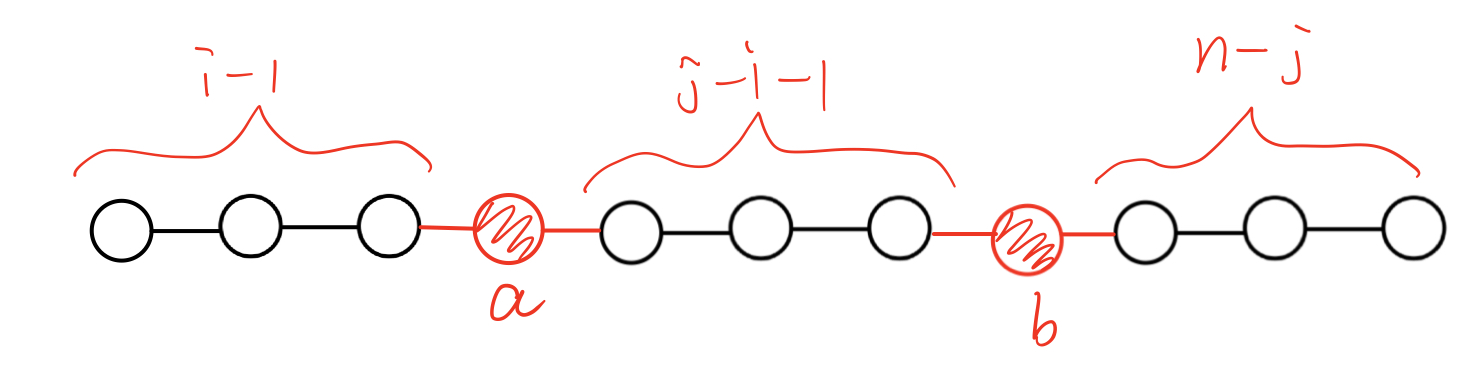
\includegraphics[width=6.2in, keepaspectratio]{1.jpeg}

To have $X_{(i)}$ be in a $\varepsilon-$interval around $a$ and  $X_{(j)}$ be in a $\varepsilon-$interval around $b$, where $a<b$.

For all these r.v.s. there are one in the $\varepsilon-$interval around $a$, and then another one in the  $\varepsilon-$interval around $b$, $i-1$ of them left of $a$, $j-i-1$ of them between $a$ and $b$, and $n - j$ of them right to $b$.

So we have$$f_{X_{(i)}, X_{(j)}}(a, b) = \frac{n!}{(i-1)!(j-i-1)!(n-j)!}(F(a))^{i-1}f(a)(F(b)-F(a))^{j-i-1}f(b)(1-F(b))^{n-j}$$
For $a<b$, otherwise $0$.

\vspace{0.4cm}
The coeff in front of it is given by the cases of choice. There are $n$ possible choices for who is at $a$ and $n-1$ possible choices for who is at $b$, etc. So the factor is $n(n-1)\binom{n-2}{i-1}\binom{n-i-1}{j-i-1}$. Other factors of this expression are given by their CDFs and PDFs.




\end{document}